\documentclass[a4paper,english]{article}
%\usepackage[T1]{fontenc}		% la font bien
\usepackage[utf8]{inputenc}		% les accents
\usepackage[french]{babel}		% la langue
\usepackage{amsmath,amssymb}	% math
\usepackage{graphicx,color,import,float,subcaption}  % graph
\usepackage[usenames,dvipsnames]{xcolor}
\usepackage[margin=2cm]{geometry} % marges
\usepackage{multicol,multirow}	% tables
\usepackage{todonotes}			% penses-bêtes
\usepackage{wrapfig}			% figures sur le côté
\usepackage{hyperref}			% liens vers les figures et formules
\usepackage{lipsum, comment}
\usepackage{listings}			% pour mettre du code

\renewcommand{\thesubfigure}{\roman{subfigure}} 
% Numérotation romaine des sous-figures pour éviter collision avec légende

\lstloadlanguages{Matlab}%
\lstset{language=Matlab,                        % Use MATLAB
        frame=single,                           % Single frame around code
        basicstyle=\small\ttfamily,             % Use small true type font
        keywordstyle=[1]\color{Blue}\bf,        % MATLAB functions bold and blue
        keywordstyle=[2]\color{Purple},         % MATLAB function arguments purple
        keywordstyle=[3]\color{Blue}\underbar,  % User functions underlined and blue
        identifierstyle=,                       % Nothing special about identifiers
                                                % Comments small dark green courier
        commentstyle=\usefont{T1}{pcr}{m}{sl}\color{MyDarkGreen}\small,
        stringstyle=\color{Purple},             % Strings are purple
        showstringspaces=false,                 % Don't put marks in string spaces
        tabsize=3,                              % 5 spaces per tab
        %
        %%% Put standard MATLAB functions not included in the default
        %%% language here
        morekeywords={xlim,ylim,var,alpha,factorial,poissrnd,normpdf,normcdf},
        %
        %%% Put MATLAB function parameters here
        morekeywords=[2]{on, off, interp},
        %
        %%% Put user defined functions here
        morekeywords=[3]{FindESS, homework_example},
        %
        morecomment=[l][\color{Blue}]{...},     % Line continuation (...) like blue comment
        numbers=left,                           % Line numbers on left
        firstnumber=1,                          % Line numbers start with line 1
        numberstyle=\tiny\color{Blue},          % Line numbers are blue
        stepnumber=1                        % Line numbers go in steps of 5
        }
\newcommand{\matlabscript}[2]
  {\begin{itemize}\item[]\lstinputlisting[caption=#2,label=#1]{#1.m}\end{itemize}}

\begin{document}

\title{Potentiel chimique d'un gaz de Bosons}
\author{Mario Geiger}
\date{\today}
\maketitle

\section{Introduction}

Sans véritable preuve mathématique, je suppose que l'intégrale ne prend pas en compte le premier terme de la somme. Donc je le rajoute :

$$N = \frac{1}{e^{-\beta \mu} - 1} + \frac{2 \pi V}{h^3} (2m)^{3/2} \int_0^\infty \frac{\sqrt{E} dE}{e^{\beta(E-\mu)}-1}$$

La température critique $T_c$ est telle que : 
$$N = \frac{2 \pi V}{h^3} (2m)^{3/2} \int_0^\infty \frac{\sqrt{E} dE}{e^{\frac{E}{k_B T_c}}-1}$$
$$\Rightarrow k_B T_c = \frac{4 \pi}{\zeta(3/2)^\frac{2}{3}} \frac{\hbar^2}{2m} \rho^\frac{2}{3}$$

\section{Adimensionnalisation}

Comme la discussion porte sur le changement de phase à la température critique, on pose $\mu = u k_B T_c$ et $T = \tau T_c$. On se retrouve alors avec :

$$N = \frac{1}{e^{-\frac{u}{\tau}} -1 } + \frac{2N}{\sqrt{\pi} \zeta(3/2)} \int_0^\infty \frac{\sqrt{x} dx}{e^{\frac{x-u}{\tau}}-1}$$

\section{Résolution numérique}
Il reste alors à trouver $u$ en fonction de $\tau$ en fixant $N$.

\matlabscript{bose}{Code matlab}

\begin{figure}
	\centering
	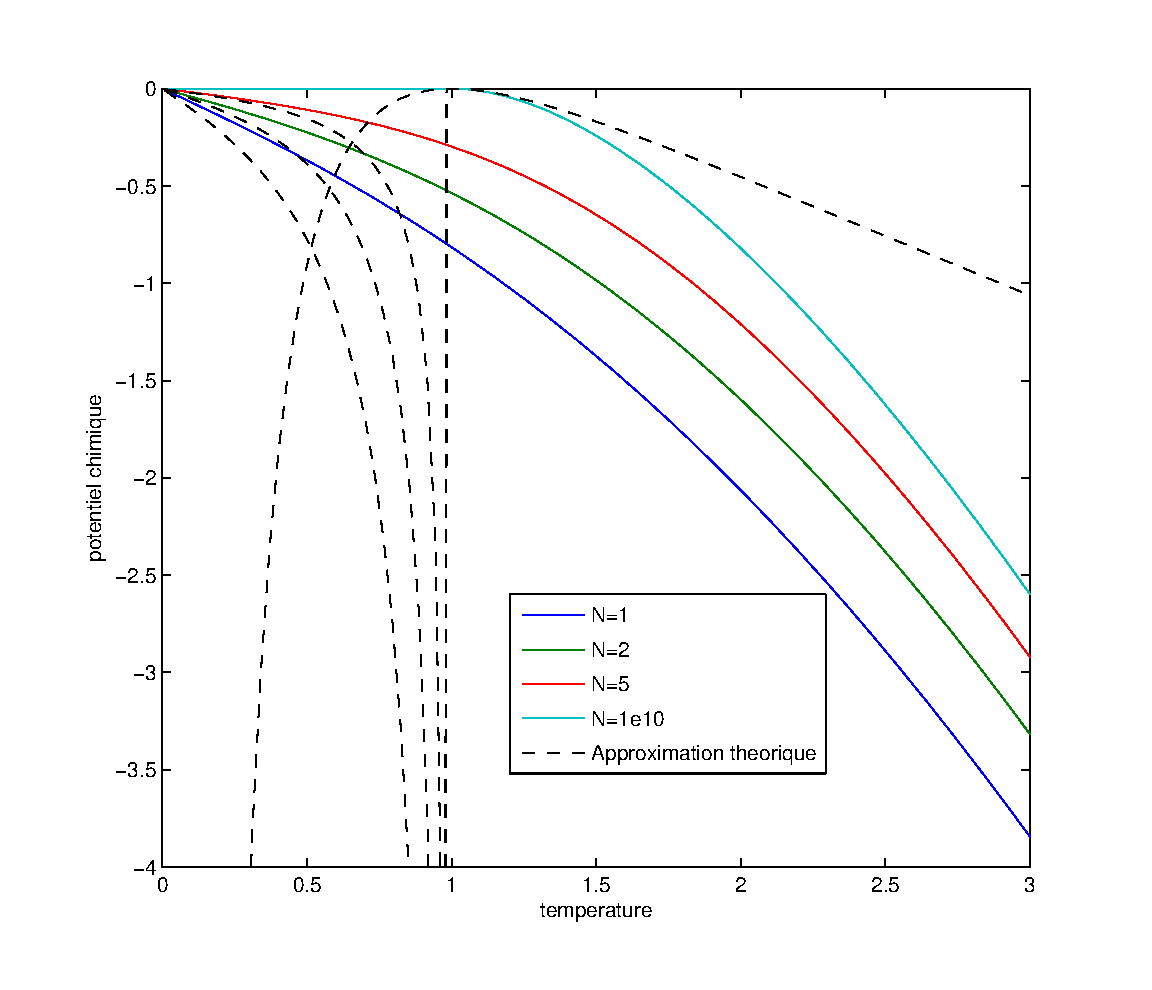
\includegraphics{untitled.eps}
	\caption{Le potentiel chimique en fonction du nombre de Bosons.}
\end{figure}


\end{document}
